% Springer Nature journal article. The class and reference style (sn-jnl.cls, sn-mathphys-num.bst) are in this project;
% SOURCE.txt says where they come from. Other reference styles: see the Springer Nature template documentation.
\documentclass[pdflatex,sn-mathphys-num]{sn-jnl}
\usepackage{graphicx}
\usepackage{amsmath,amssymb}
\usepackage{booktabs}

\begin{document}

% Replace with your title; the optional argument is the short title for page headers.
\title[Sleep Duration from Charging Patterns]{Estimating Sleep Duration from Smartphone Charging Patterns: A Validation Study}

% Authors: * marks the corresponding author, the number links to an affiliation below.
\author*[1]{\fnm{Hannah} \sur{Keller}}\email{hannah.keller@altmark.example}
\author[1,2]{\fnm{Rohan} \sur{Deshpande}}\email{rohan.deshpande@altmark.example}
\author[2]{\fnm{Lucia} \sur{Moretti}}\email{lucia.moretti@sleepclinic.example}

\affil*[1]{\orgdiv{Department of Public Health}, \orgname{Altmark University}, \orgaddress{\city{Magdeburg}, \country{Germany}}}
\affil[2]{\orgdiv{Sleep Medicine Unit}, \orgname{St. Clara Hospital}, \orgaddress{\city{Turin}, \country{Italy}}}

% Replace with your abstract.
\abstract{Large studies of sleep rely on questionnaires, which overestimate sleep duration, or on wearable devices, which many participants stop using within weeks. We tested whether the times at which people plug in and unplug their smartphone can stand in for both. For 28 nights, 164 adults wore a wrist actigraph and ran an app that recorded charging events and screen use. An estimate based on the longest overnight period without screen use, anchored by charging times, differed from actigraphy by a mean of 11 minutes, with 95\% limits of agreement from $-52$ to 74 minutes. Agreement was better than for self-report, which overestimated sleep by 38 minutes on average. The method needs no additional device and may be suitable for studies in which weekly averages, rather than single nights, are of interest.}

\keywords{Sleep duration, Smartphone, Actigraphy, Digital phenotyping, Validation}

\maketitle

\section{Introduction}\label{sec:introduction}
Short and irregular sleep is associated with cardiovascular disease, depression and accidents, and public-health research therefore needs to measure sleep in large groups over long periods. The reference method outside the laboratory is actigraphy, in which a wrist-worn accelerometer infers sleep from the absence of movement~\cite{sadeh2011role}. It is accurate, but devices are costly and participants tire of wearing them.

Questionnaires such as the Pittsburgh Sleep Quality Index~\cite{buysse1989pittsburgh} cost little and scale well. People tend, however, to report the time they spend in bed rather than the time they sleep, and self-reported duration exceeds measured duration by half an hour or more~\cite{lauderdale2008self}.

Smartphones offer a third source. Most adults keep one within reach at night and many charge it while they sleep. This study asks how well sleep duration can be estimated from charging and screen events alone, compared with actigraphy. Sect.~\ref{sec:methods} describes the participants and the estimate, Sect.~\ref{sec:results} the agreement between methods, and Sect.~\ref{sec:discussion} the limits of the approach.

\section{Methods}\label{sec:methods}
\subsection{Participants}
We recruited 164 adults aged 19 to 67 years (mean 38.4, 55\% women) through a university panel. Shift workers and people with a diagnosed sleep disorder were not included. The study was approved by the ethics committee of Altmark University, and all participants gave written consent.

\subsection{Procedure}
Fig.~\ref{fig:workflow} outlines the study. Participants wore an actigraph on the non-dominant wrist for 28 consecutive nights and installed an app that logged the time of every charging and screen event. Each morning they reported the previous night's sleep duration in a one-question diary.

\begin{figure}[t]
  \centering
  % Replace with your own figure: upload an image and change the file name below.
  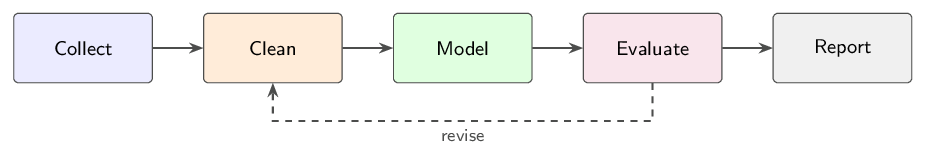
\includegraphics[width=0.9\textwidth]{figures/workflow.png}
  \caption{Stages of the study, from data collection to reporting. Estimates were revised once, after the first 40 participants, before the main analysis.}
  \label{fig:workflow}
\end{figure}

\subsection{Estimating sleep from the phone}
For each night we took the longest interval without screen use between 20:00 and 11:00. If the phone was plugged in within 30 minutes before that interval began, the plug-in time replaced its start. The estimated sleep duration is
\begin{equation}\label{eq:estimate}
  \hat{d} = (t_{\mathrm{end}} - t_{\mathrm{start}}) - \delta ,
\end{equation}
where $t_{\mathrm{start}}$ and $t_{\mathrm{end}}$ bound the interval and $\delta = 19$ minutes is the mean time to fall asleep in the first 40 participants, who were excluded from the validation.

\subsection{Statistical analysis}
Agreement with actigraphy was assessed with the mean difference and 95\% limits of agreement. Nights with fewer than four hours of actigraph wear were excluded, leaving 3\,214 nights from 124 participants.

\section{Results}\label{sec:results}
Table~\ref{tab:agreement} compares the phone-based estimate and the diary with actigraphy. The phone-based estimate exceeded actigraphy by 11 minutes on average, the diary by 38 minutes. The limits of agreement for single nights were wide for both methods, but when nights were averaged per participant and week the limits for the phone-based estimate narrowed to $-21$ and 43 minutes.

\begin{table}[t]
\caption{Agreement of two methods with actigraphy. Differences are method minus actigraphy, in minutes.}\label{tab:agreement}
\begin{tabular}{@{}lccc@{}}
\toprule
Method & Mean difference & Limits of agreement & Correlation \\
\midrule
Phone-based, single nights & 11 & $-52$ to 74 & 0.81 \\
Phone-based, weekly means  & 11 & $-21$ to 43 & 0.92 \\
Diary, single nights       & 38 & $-49$ to 125 & 0.64 \\
Diary, weekly means        & 38 & $-12$ to 88 & 0.77 \\
\botrule
\end{tabular}
\end{table}

The estimate was least accurate for the 17 participants who did not charge their phone overnight on most nights; among them the mean difference was 29 minutes. Age and sex were not associated with the size of the error.

\section{Discussion}\label{sec:discussion}
Charging and screen events recover sleep duration more closely than a morning diary does, and without asking participants to wear or do anything. The error on a single night is too large for clinical use, which matches what is known about actigraphy's own limits~\cite{sadeh2011role}. For weekly means, which are what cohort studies usually analyse, agreement was good.

The method depends on habits. It fails for people who do not keep their phone nearby at night and overestimates sleep for those who lie awake without touching it. Our participants were volunteers from a university panel, and agreement may be lower in other groups.

\section{Conclusion}\label{sec:conclusion}
Smartphone charging and screen events give an estimate of sleep duration that agrees with actigraphy to within 11 minutes on average. The approach is a practical option for large studies that need weekly sleep duration and cannot provide a device to every participant.

\backmatter

\bmhead{Acknowledgements}
We thank the participants, and Jana Vogel for coordinating data collection.

\section*{Declarations}
\begin{itemize}
\item \textbf{Funding} This work was supported by the Altmark Health Research Fund (grant AHR-2024-22).
\item \textbf{Competing interests} The authors declare no competing interests.
\item \textbf{Ethics approval} Approved by the ethics committee of Altmark University (reference 2024-117).
\item \textbf{Data availability} De-identified data are available from the corresponding author on reasonable request.
\end{itemize}

\bibliography{references}

\end{document}
